\documentclass[11pt]{article}
\usepackage{graphicx}
\usepackage{subcaption}
\usepackage[table]{xcolor}
\usepackage{float}
\usepackage[a4paper,margin=2cm]{geometry}
\usepackage{fancyhdr}
\usepackage{listings}

\lstnewenvironment{rc}[1][]{\lstset{language=R}}{}
\newcommand{\ri}[1]{\lstinline{#1}}  %% Short for 'R inline'

\lstset{language=R}             % Set R to default language

\begin{document}

\title{STAT 565 HW-2}
\author{Yokesh Thirumoorthi}

\maketitle
\pagestyle{fancy}
\fancyhf{}
\rhead{Yokesh Thirumoorthi}
\lhead{STAT 565 HW-2 Winter 2020}
\rfoot{Page \thepage}

\section{Question 1}

\paragraph{Data Processing}
In order to carry out data analyses with R, the given data is formatted to two columns - one for independent variable (Mixing Technique) and another for the dependent variable (Tensile Strength). With this data format, the data is easily read with read.table() function in R.

\begin{lstlisting}[language=R]
    datafilename="./data/hw1.data"
    #read the data into a table
    data=read.table(datafilename,header=T)
\end{lstlisting}

\paragraph{Analyses}
In this problem, we are given a data set with a = 4 subsets, each containing n = 4 values for a total of $\displaystyle N=an=16$ data points. 
Each subset contains measurements of tensile strength of cement samples that were produced with a different mixing technique, or treatment. We define the mean over all data points as the grand mean, and the mean of each point within a given treatment as the treatment mean.

Since we are given a finite set of data, we could approximate these means by calculating sample means and compare each treatment data subset. The grand sample mean and the treatment sample means is given by: 

\begin{lstlisting}[language=R]
    # Find the grand sample mean
    mean(data$Tensile_Strength) 

    # Find the treatment sample means
    mean(data$Tensile_Strength[data$Mixing_Technique == 1])
    mean(data$Tensile_Strength[data$Mixing_Technique == 2])
    mean(data$Tensile_Strength[data$Mixing_Technique == 3])
    mean(data$Tensile_Strength[data$Mixing_Technique == 4])
    
    # Find Standard errors
    sd(data$Tensile_Strength)
    sd(data$Tensile_Strength[data$Mixing_Technique == 1])
    sd(data$Tensile_Strength[data$Mixing_Technique == 2])
    sd(data$Tensile_Strength[data$Mixing_Technique == 3])
    sd(data$Tensile_Strength[data$Mixing_Technique == 4])

\end{lstlisting}

\clearpage

\lstinputlisting[float=h,frame=tb,caption=R output,label=zebra]{../out/hw1_means.txt}

We now create a aov object

\begin{lstlisting}[language=R]
    #do the analysis of variance
    model1 = aov(Tensile_Strength~Mixing_Technique,data=data.ex1)

    #show the summary table
    summary(model1)
\end{lstlisting}

\lstinputlisting[float=h,frame=tb,caption=R output,label=zebra]{../out/hw1_anova.txt}

\subsection{Test the hypothesis that mixing techniques affect the strength of the cement. Use $\displaystyle \alpha=0.05$.}
We have to know if one of the data subsets is significantly different from the others, as this may indicate that one of our manufacturing techniques is superior (or inferior) to the others. To compare our data subsets we are interested in whether most of the error is within the treatments or between the treatments. If most of the error is between the treatment means, then we can claim there are significant differences between them. If there is too much error within the treatment means we cannot claim that they are significantly different. Using the output of ANOVA, we have found the error between the treatment means as 

$$\displaystyle MS_{Treatment} = 163,247$$

The error within the treatment means could be observed from anova summary: 

$$\displaystyle MS_{Error} = 12,826$$

And the ratio is (f-value from anova output),

$$\displaystyle F_0 = MS_{Treatment}/MS_{Error} = 12.7$$

To determine whether or not there are significant differences between our treatments, we will compare above $\displaystyle F_0$ to $\displaystyle F_{\alpha, a-1, N-a}$. $\displaystyle F_{\alpha, a-1, N-a}$ is determined in R as below,

\begin{lstlisting}[language=R]
    qf(1-0.05, 3, 12)   

    # Output
    [1] 3.490295
\end{lstlisting}

\paragraph{Conclusion}
If $\displaystyle F_{0}>F_{\alpha ,\,a-1,\,N-a}$, which is the case here, then the error between treatment means is large enough compared to the error within treatment means to conclude that there is a significant difference between at least one treatment and the others. Also the F-value is 12.73 with the coresponding P-value of 0.0005. Hence mixing technique has effect and it affects the strength of cement.

\subsection{Construct a graphical display as described in Section 3-5.3 to compare the mean tensile strengths for the four mixing techniques. What are your conclusions?}


\begin{lstlisting}[language=R]
    library(ggplot2)

    y1bar <- mean(data$Tensile_Strength[data$Mixing_Technique == 1])
    y2bar <- mean(data$Tensile_Strength[data$Mixing_Technique == 2])
    y3bar <- mean(data$Tensile_Strength[data$Mixing_Technique == 3])
    y4bar <- mean(data$Tensile_Strength[data$Mixing_Technique == 4])
    
    x <- seq(-4.5, 4.5, length = 90)
    xval <- c(y1bar, y2bar, y3bar, y4bar)
    
    xvaltrn <- (xval - mean(xval))/(sd(xval)/sqrt(3))
    tvalues <- dt(x,15)
    
    vlines <- data.frame(xint = 
        c(xvaltrn,mean(xvaltrn)),grp = letters[1:5])
    attach(vlines)
  
    qplot(x, tvalues) 
    + geom_polygon(fill = "white", colour = "grey", alpha = 0.2)  
    + geom_vline(data = vlines, aes(xintercept = xint, colour = grp), 
                linetype = "dashed", size = 0.5) 
    + theme_bw() 
    + xlab((('x values with intercept of Average Tensile Strength'))) 
    + ylab(expression(bold(P(x))))

\end{lstlisting}

\begin{figure}[H]
    \centering
    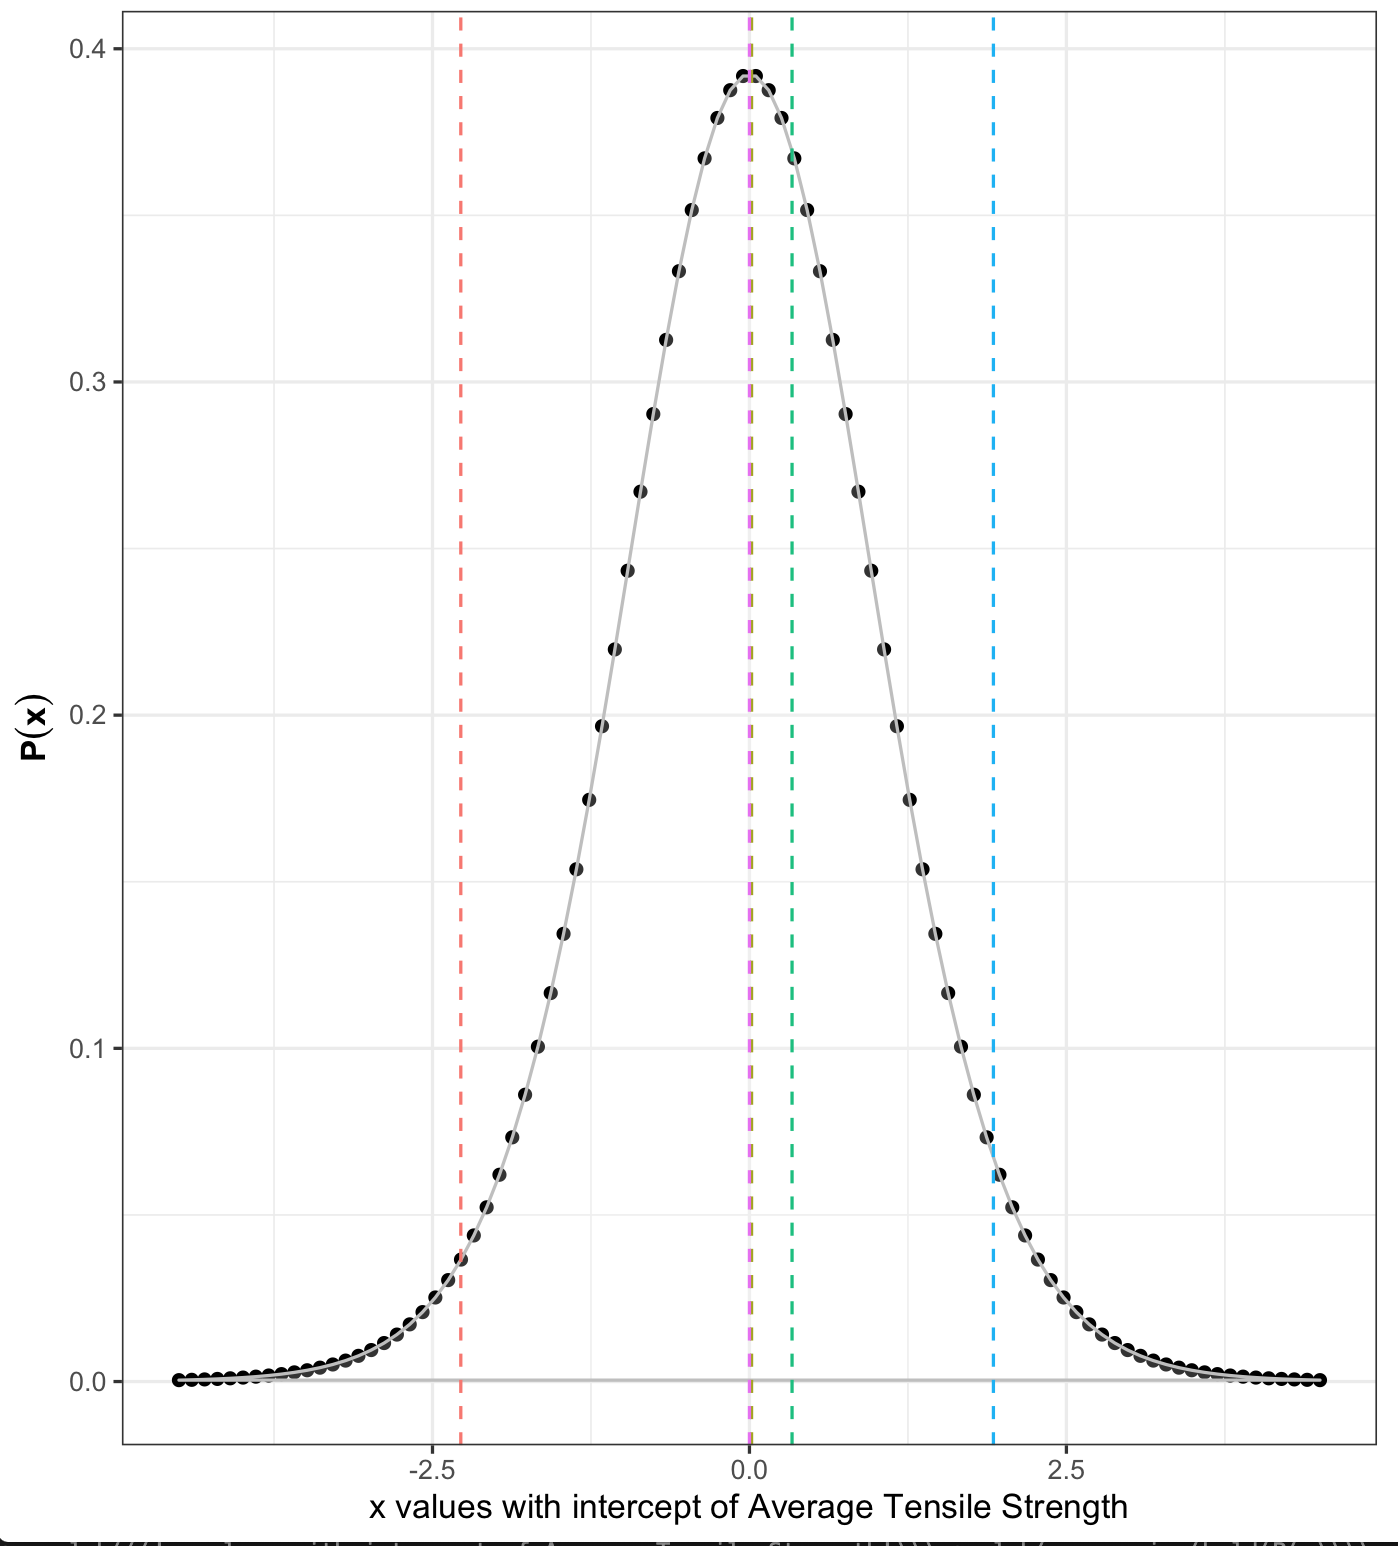
\includegraphics[width=3.0in]{../pictures/hw2_q1_b.png}
    \caption{t-Distribution}
    \label{t-Distribution}
\end{figure}


\paragraph{Conclusion}
Based on examination of the plot, we would conclude that 
$\displaystyle \mu_1$ and $\displaystyle \mu_3$ are the same.
$\displaystyle \mu_4$ differs from $\displaystyle \mu_1$ and $\displaystyle \mu_3$;
$\displaystyle \mu_2$ differs from $\displaystyle \mu_1$ and $\displaystyle \mu_3$;
$\displaystyle \mu_4$ and $\displaystyle \mu_2$ are differnt;


\subsection{Use the Fisher LSD method with $\displaystyle \alpha=0.05$ to make comparisons between pairs of means.}

Fisher LSD comparisons allow each pair of treatment means to be compared. 
If $\displaystyle \mid \bar{y_i} - \bar{y_j} \mid > LSD$ then the treatment means  $\displaystyle i$ and $\displaystyle j$ are significantly different. 

From section1.1 above, we have the treatment means as 
$\displaystyle \bar{y_1.}=2971, \bar{y_2.}=3156.25, \bar{y_3.}=2933.75, \bar{y_4.}=2666.25$

\paragraph{}
\begin{tabular}{ |p{1cm}|p{1cm}|p{1cm}|p{1cm}|p{1cm}|  }
    \hline
    \multicolumn{5}{|c|}{$\displaystyle \mid \bar{y_i} - \bar{y_j} \mid$ } \\
    \hline
     - & 1 & 2 & 3 & 4 \\ \hline
    1 & - & \cellcolor{gray!30} 185.25 & 22.75 & \cellcolor{gray!30}304.75 \\ \hline
    2 & \cellcolor{gray!30} 185.25 & - & 162.5 & \cellcolor{gray!30}490 \\ \hline
    3 & 22.75 & 162.5 & - & \cellcolor{gray!30}327.5 \\ \hline
    4 & \cellcolor{gray!30}304.75 & \cellcolor{gray!30}490 & \cellcolor{gray!30}327.5 & - \\ \hline
\end{tabular}

\paragraph{}
Using the below R program, we got the LSD = 174.479.

The pair of treatment averages that differ in absolute value by more than 174.479 are {1 and 2}, {1 and 4}, {2 and 4} and {3 and 4}.
And it would imply that there is a statistically significant difference between these treatment.

\clearpage

\begin{lstlisting}[language=R]
    library(agricolae)
    lsd <- LSD.test(model1,"Mixing_Technique")
    lsd
\end{lstlisting}

\lstinputlisting[float=h,frame=tb,caption=R output,label=zebra]{../out/hw2_fisher.txt}

   
\clearpage

\subsection{Construct a normal probability plot of the residuals. What conclusion would you draw about the validity of the normality assumption?}

Inorder to verify that the residuals are normally distributed in our experiment, we use
normal-normal quantail plot. 


\begin{figure}[H]
    \centering
    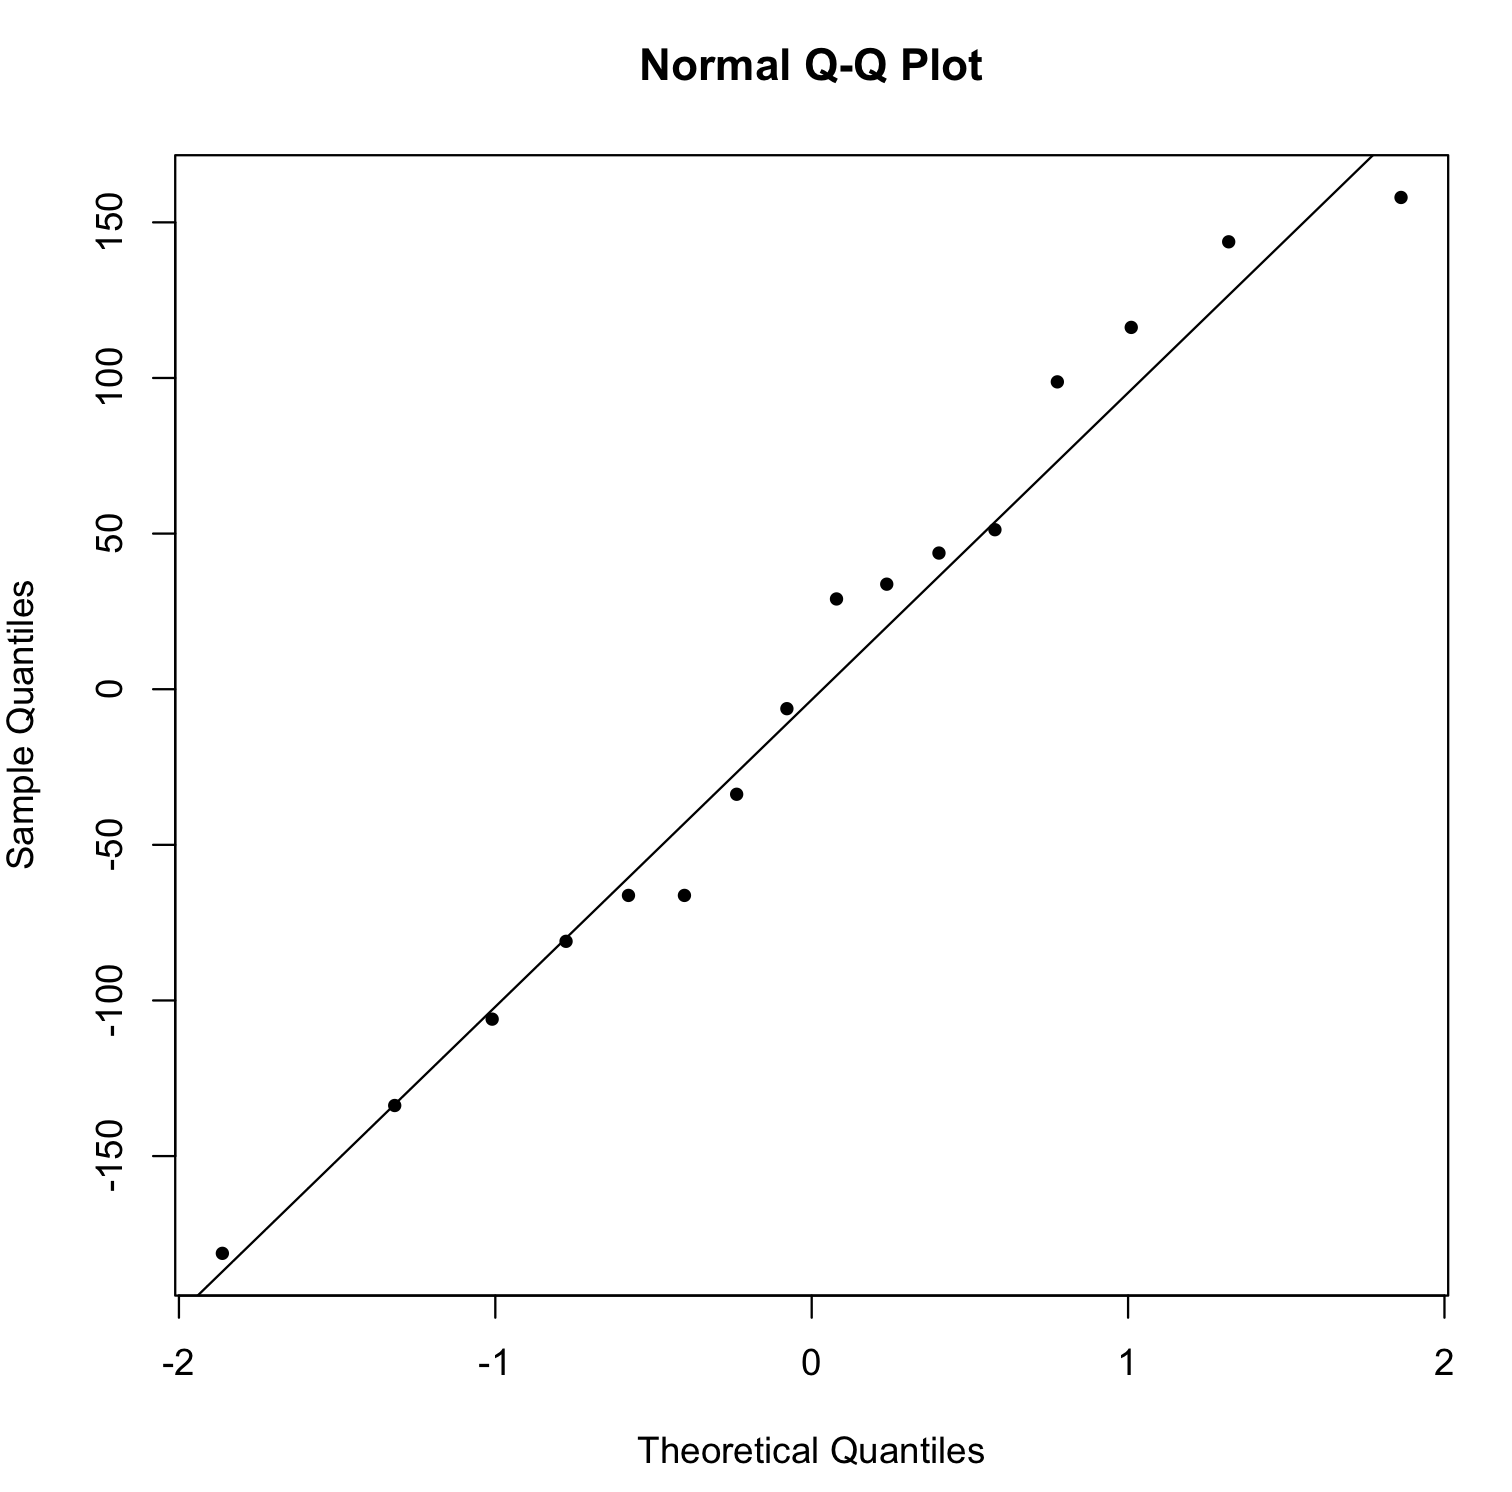
\includegraphics[width=3.0in]{../pictures/hw2_q1_qqplot.png}
    \caption{Q-Q Plot}
    \label{Q-Q Plot}
\end{figure}

There does not seem to be a problem with normality as the plots are generally in a straight line.

\subsection{Plot the residuals versus the predicted tensile strength. Comment on the plot.}

As an estimate of the tensile strength for each treatment, we use the treatment mean. The plot of residuals vs. their treatment means gives an indication of the relative sizes of errors between (x-axis) and within (y-axis) treatments. 

\begin{figure}[H]
    \centering
    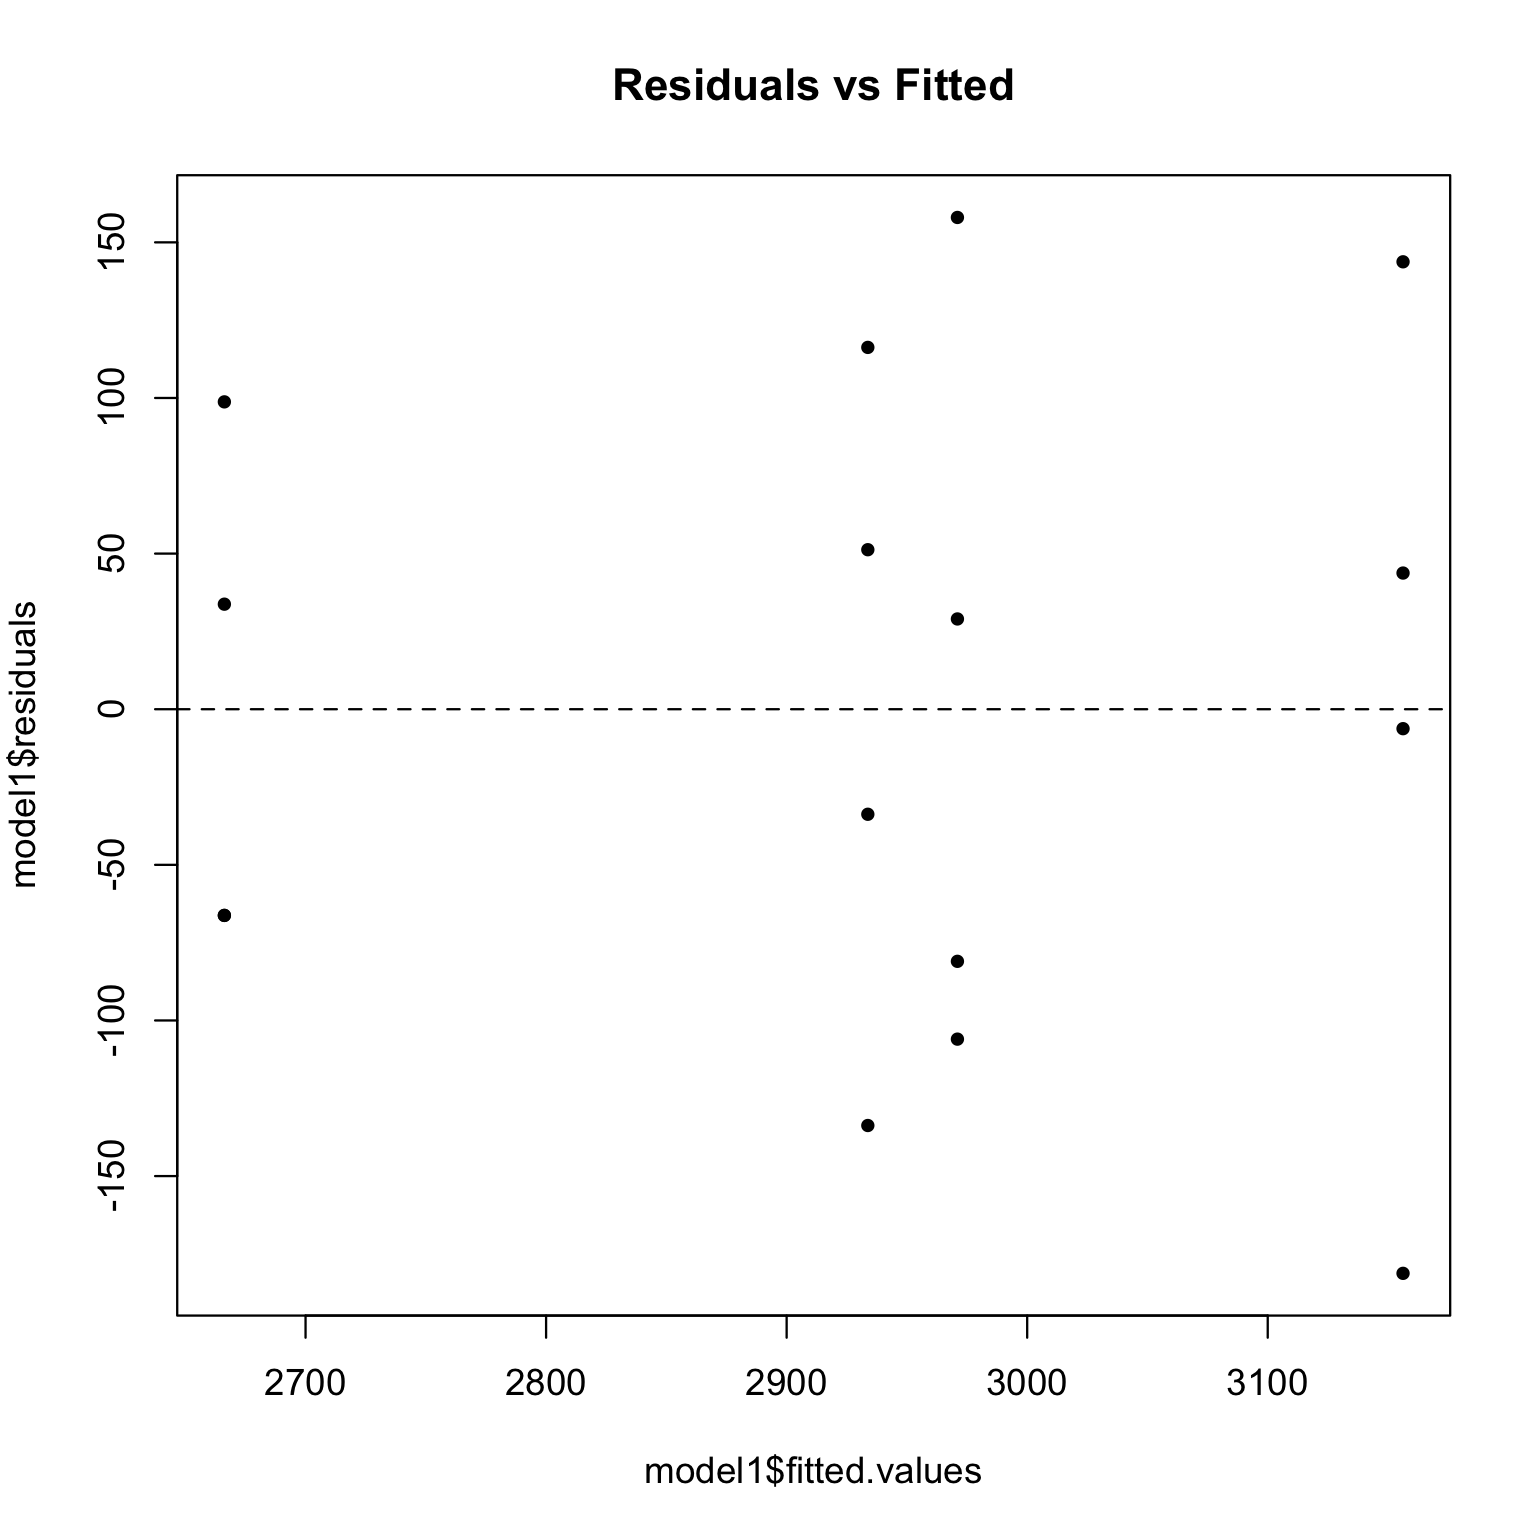
\includegraphics[width=3.0in]{../pictures/hw2_q1_pf.png}
    \caption{Residuals vs Fitted plot}
    \label{Residuals vs Fitted plot}
\end{figure}


The plots are relatively shapeless and there is no linear pattern. The residuals are almost equally distributed around the 0 line without large outliers.


\subsection{Prepare a scatter plot of the results to aid the interpretation of the results of this experiment}

\begin{figure}[H]
    \centering
    \begin{subfigure}{0.45\textwidth}
        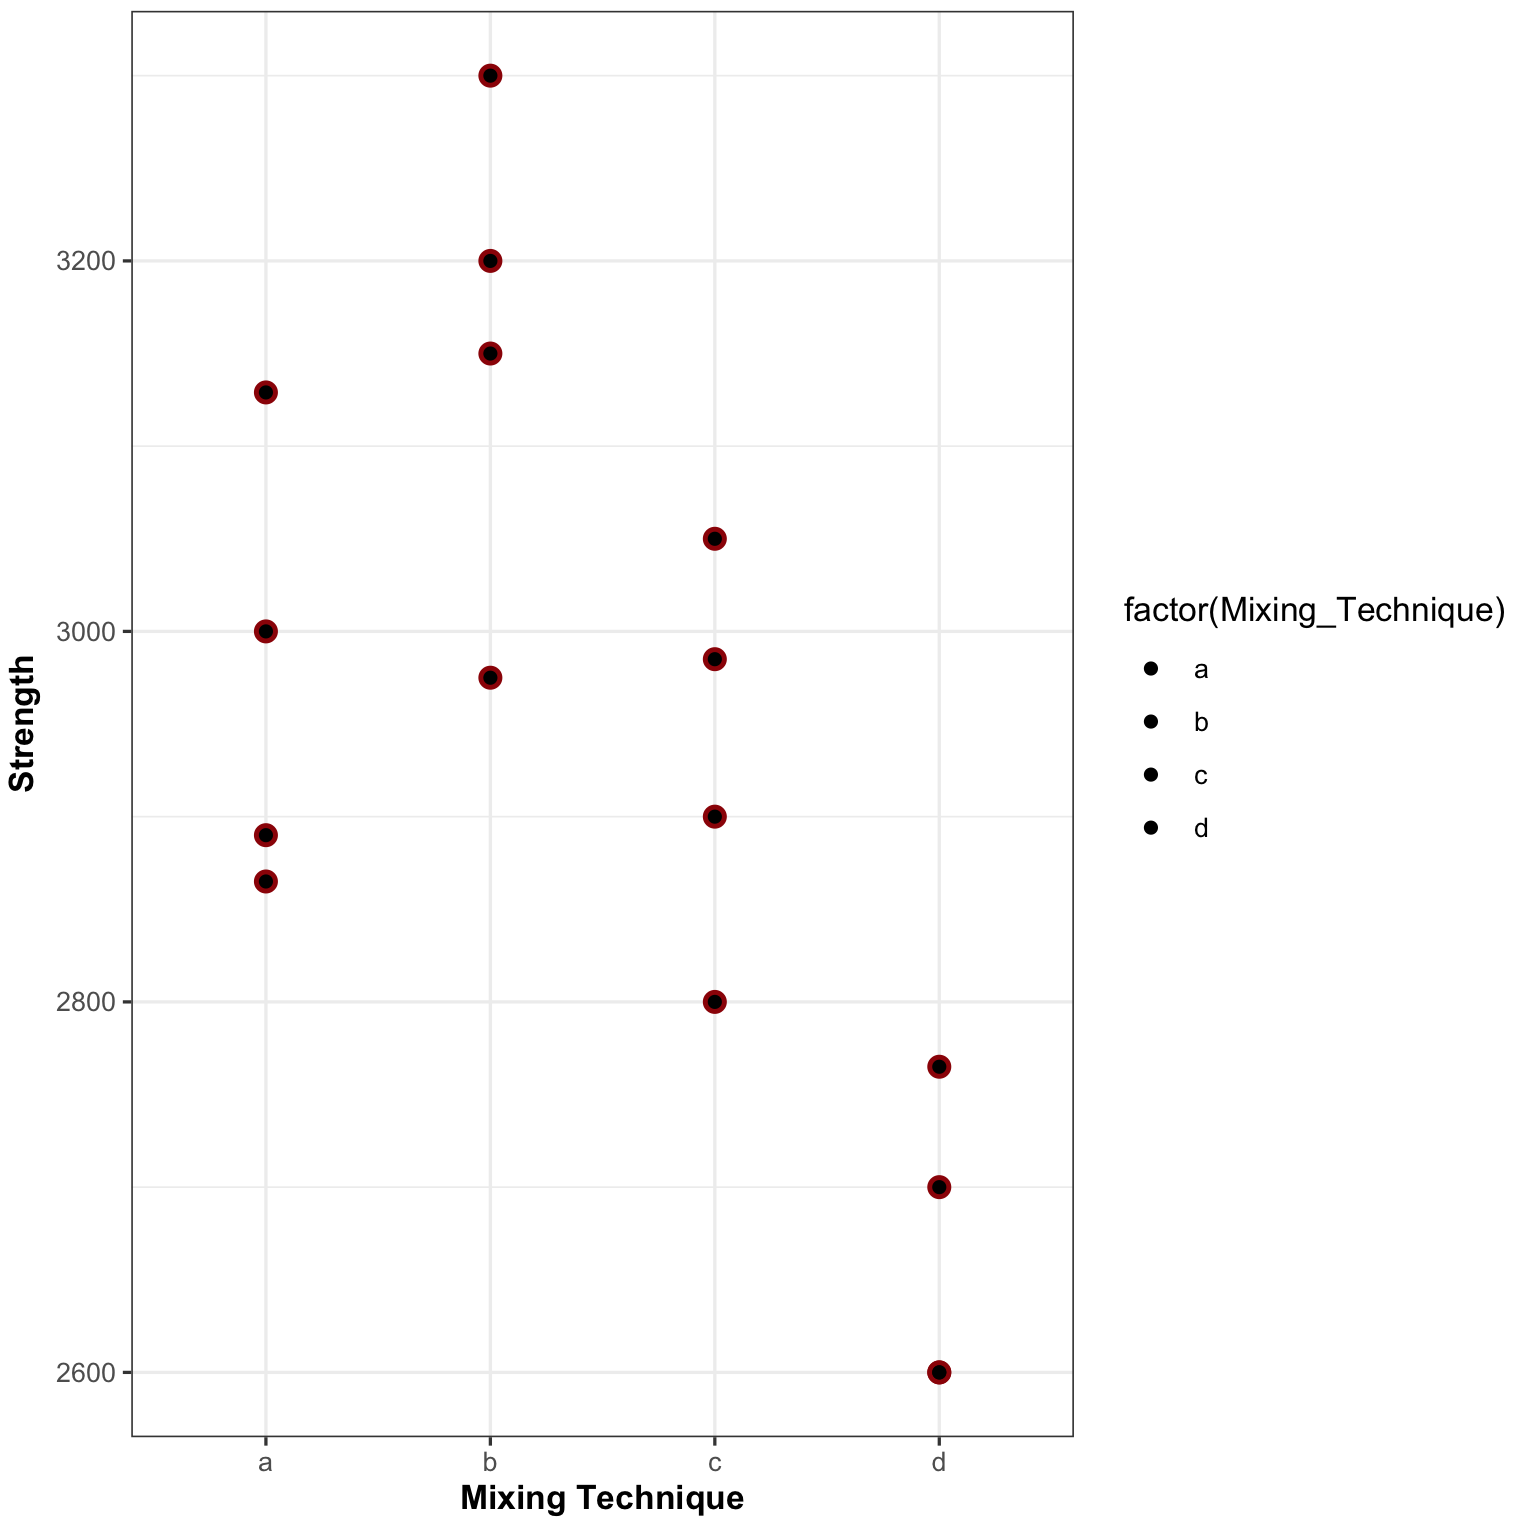
\includegraphics[width=\textwidth]{../pictures/hw2_q1_scatter.png}
        \caption{Scatter Plot}
    \end{subfigure}
    \begin{subfigure}{0.45\textwidth}
        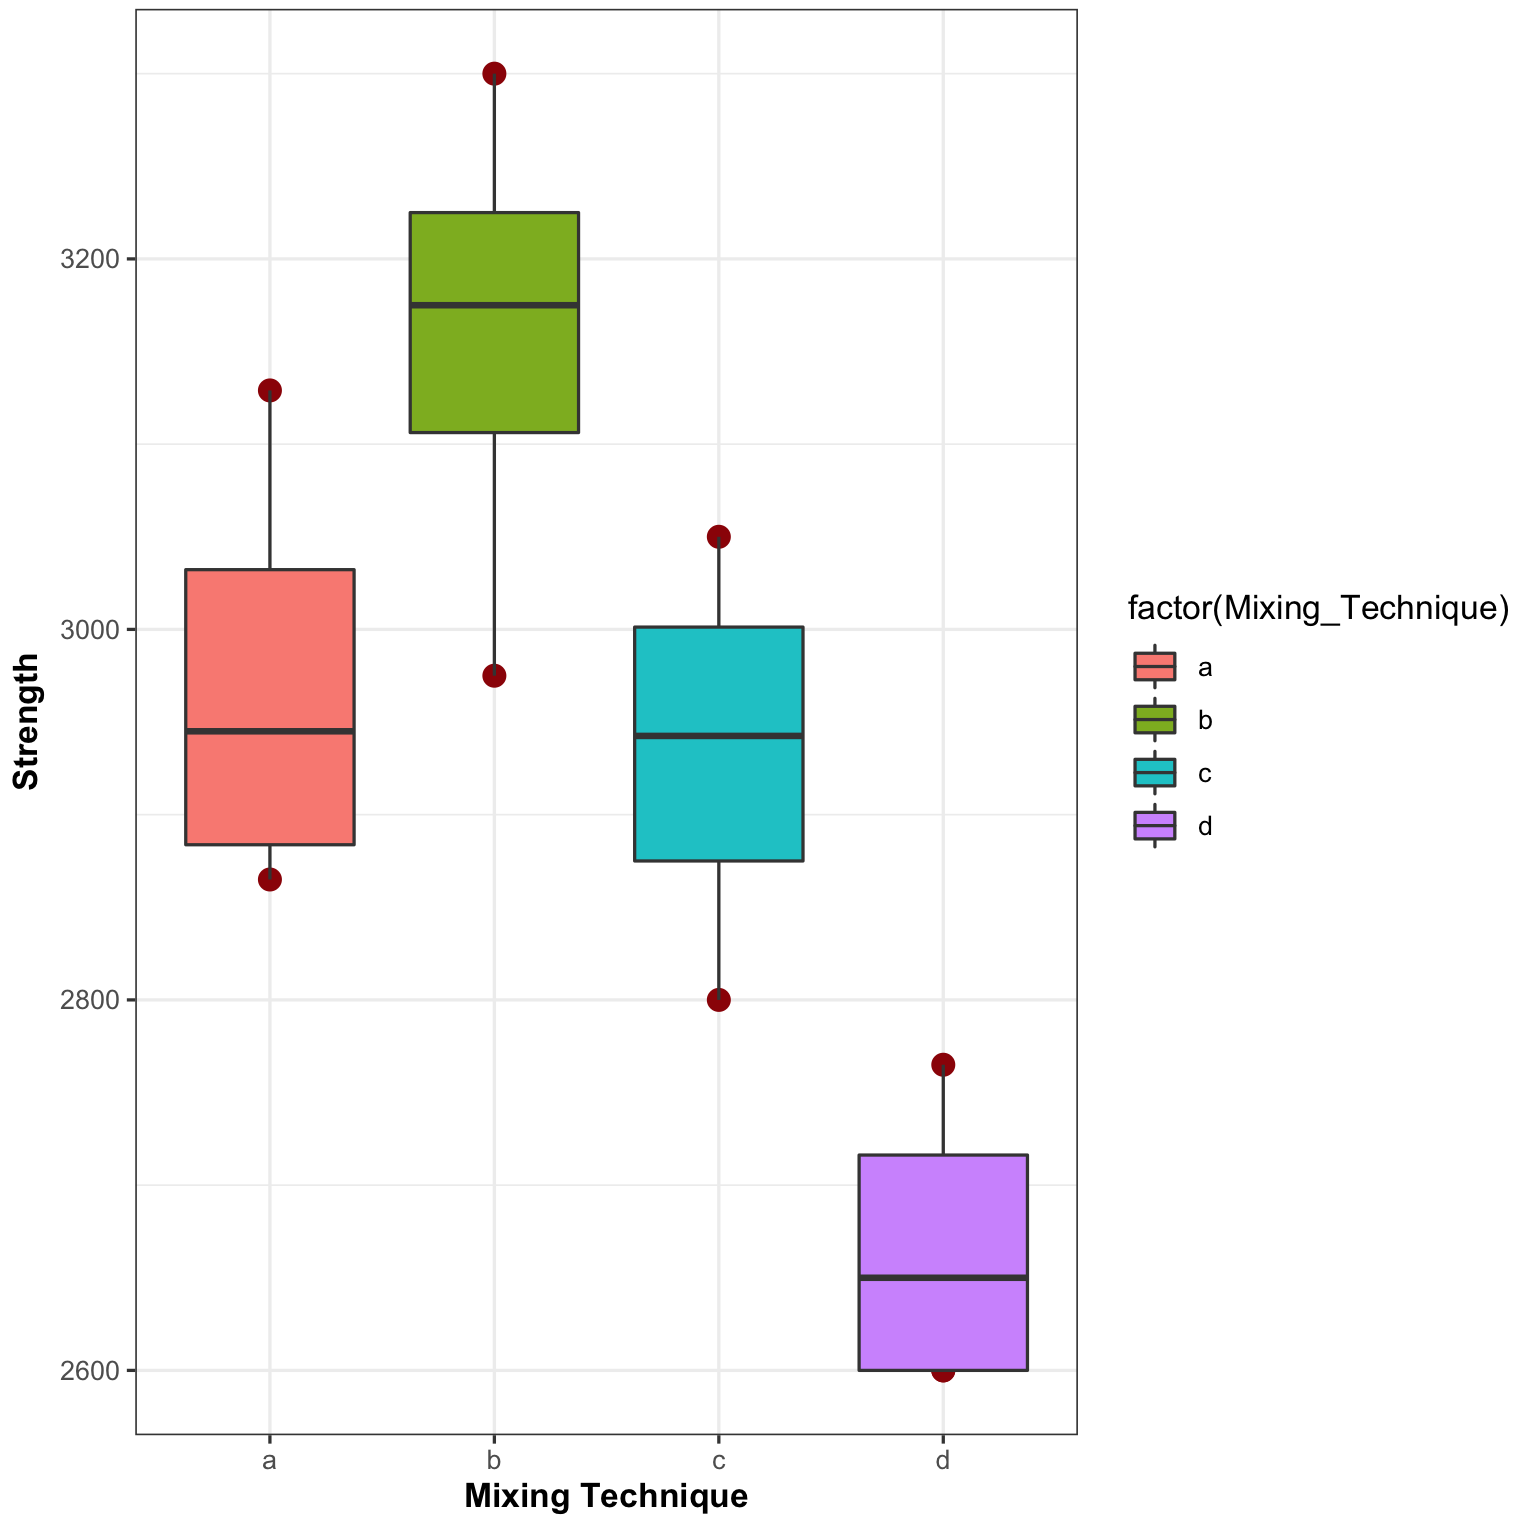
\includegraphics[width=\textwidth]{../pictures/hw2_q1_box.png}
        \caption{Box Plot}
    \end{subfigure}
\end{figure}

\clearpage
% % % % % % % % % % % % % % % % % % % % % % % % % % % % % % % % % % % % % % % 
% % % %                 Question 2                              % % % % % % % 
% % % % % % % % % % % % % % % % % % % % % % % % % % % % % % % % % % % % % % % 
\section{Question 2}

\paragraph{Data Processing}
The given data is formatted to two columns - one for the dependent variable (observations) and another for the independent variable (dosage). With this data format, the data is easily read with read.table() function in R.

\begin{lstlisting}[language=R]
    datafilename="./data/hw2.data"
    #read the data into a table
    data=read.table(datafilename,header=T)
\end{lstlisting}


\paragraph{Analyses}
In this problem, we are given a data set with a = 3 subsets, each containing n = 4 values for a total of $\displaystyle N=an=12$ data points. 

\begin{lstlisting}[language=R]
    #do the analysis of variance
    model2 = aov(Observations~Dosages,data=data)

    #show the summary table
    summary(model2)
\end{lstlisting}

\lstinputlisting[float=h,frame=tb,caption=R output,label=zebra]{../out/hw1_anova_q2.txt}

\subsection{Is there evidence to indicate that dosage level affects bioactivitys}
We have to know if one of the data subsets is significantly different from the others, as this may indicate that one of the treatment is superior (or inferior) to the others. To compare our data subsets we are interested in whether most of the error is within the treatments or between the treatments. If most of the error is between the treatment means, then we can claim there are significant differences between them. If there is too much error within the treatment means we cannot claim that they are significantly different. Using the output of ANOVA, we have found the error between the treatment means as 

$$\displaystyle MS_{Treatment} = 225.33$$

The error within the treatment means could be observed from anova summary: 

$$\displaystyle MS_{Error} = 32.03$$

And the ratio is (f-value from anova output),

$$\displaystyle F_0 = MS_{Treatment}/MS_{Error} = 7.04$$

To determine whether or not there are significant differences between our treatments, we will compare above $\displaystyle F_0$ to $\displaystyle F_{\alpha, a-1, N-a}$. $\displaystyle F_{\alpha, a-1, N-a}$ is determined in R as below,

\begin{lstlisting}[language=R]
    qf(1-0.05, 2, 9)   

    # Output
    [1] 4.256495
\end{lstlisting}

\paragraph{Conclusion}
If $\displaystyle F_{0}>F_{\alpha ,\,a-1,\,N-a}$, which is the case here, then the error between treatment means is large enough compared to the error within treatment means to conclude that there is a significant difference between at least one treatment and the others. Also the F-value is 7.04 with the coresponding P-value of 0.01. Hence there appears to be a difference in dosages.

\subsection{If it is appropriate to do so, make comparisions between the pairs of means. What conclusion can you draw?}

Since we are given a finite set of data, we could calculate sample means and compare each dosages data subset. The grand sample mean and the dosages sample means is given by: 

\begin{lstlisting}[language=R]
    
    mean(data$Observations)
    mean(data$Observations[data$Dosages == 20])
    mean(data$Observations[data$Dosages == 30])
    mean(data$Observations[data$Dosages == 40])

    model2 = aov(Observations~Dosages,data=data)    
    lsd <- LSD.test(model2,"Dosages")
    lsd

\end{lstlisting}

\clearpage

\lstinputlisting[float=h,frame=tb,caption=R output,label=zebra]{../out/hw1_means_q2.txt}

\begin{center}
    \begin{tabular}{ | c | r |}
      \hline
                         & $\displaystyle \mid \bar{y_i} - \bar{y_j} \mid$ \\ \hline
       Treatment a and b & 7 \\ \hline
       Treatment a and c & \cellcolor{gray!30}15 \\ \hline
       Treatment b and c & 8 \\ \hline
    \end{tabular}
\end{center}
Here Treatment a is dosage 20g, Treatment b is dosage 30g and Treatment c is dosage 40g
\paragraph{}
Because there appears to be a difference in the dosages, the comparision of means is appropriate.
And by doing a Fisher comparision, we could notice that there is a significant
difference between dosage 20g and 40g.

\subsection{Analyse the residuals from this experiment and comment on the model adequecy}

\begin{figure}[H]
    \centering
    \begin{subfigure}{0.45\textwidth}
        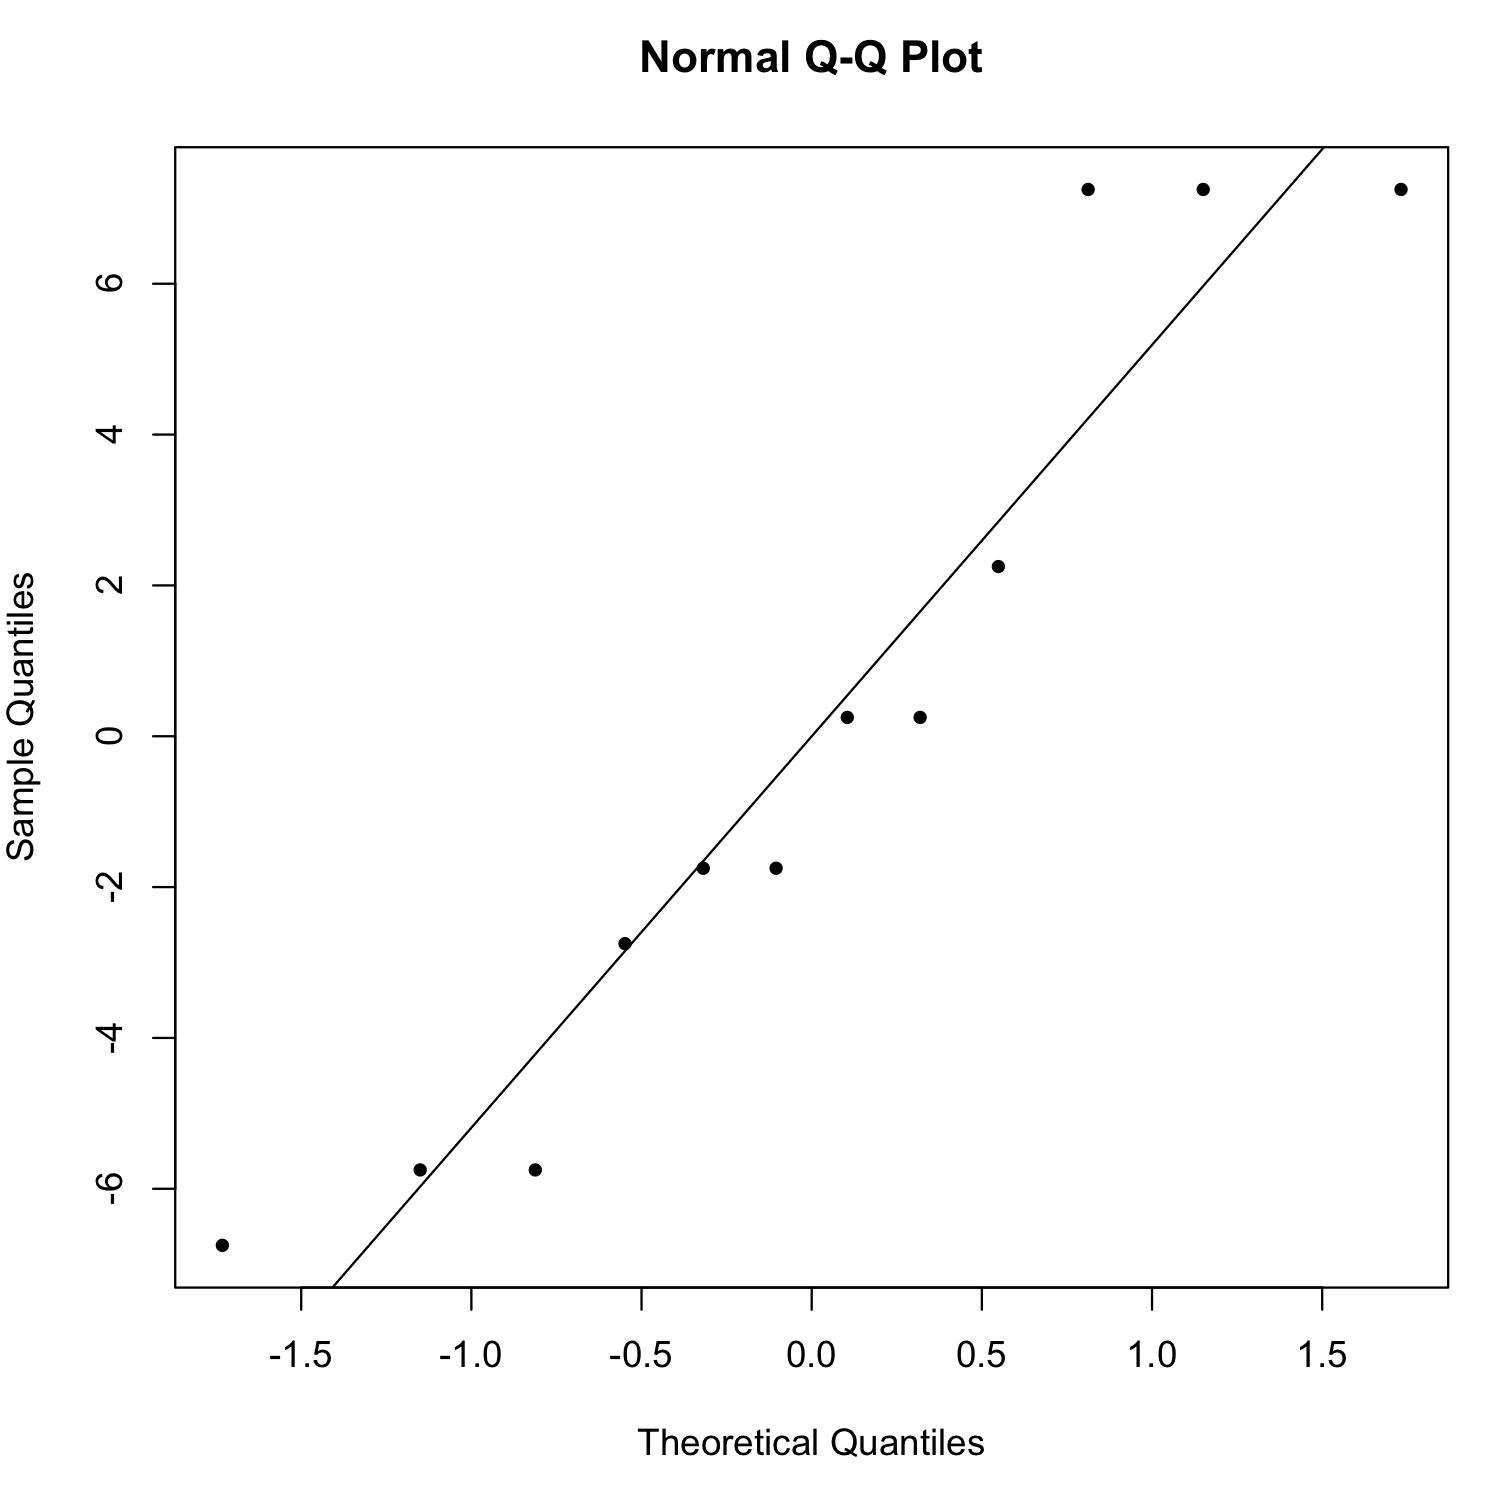
\includegraphics[width=\textwidth]{../pictures/hw2_q2_qq.png}
    \end{subfigure}
    \begin{subfigure}{0.45\textwidth}
        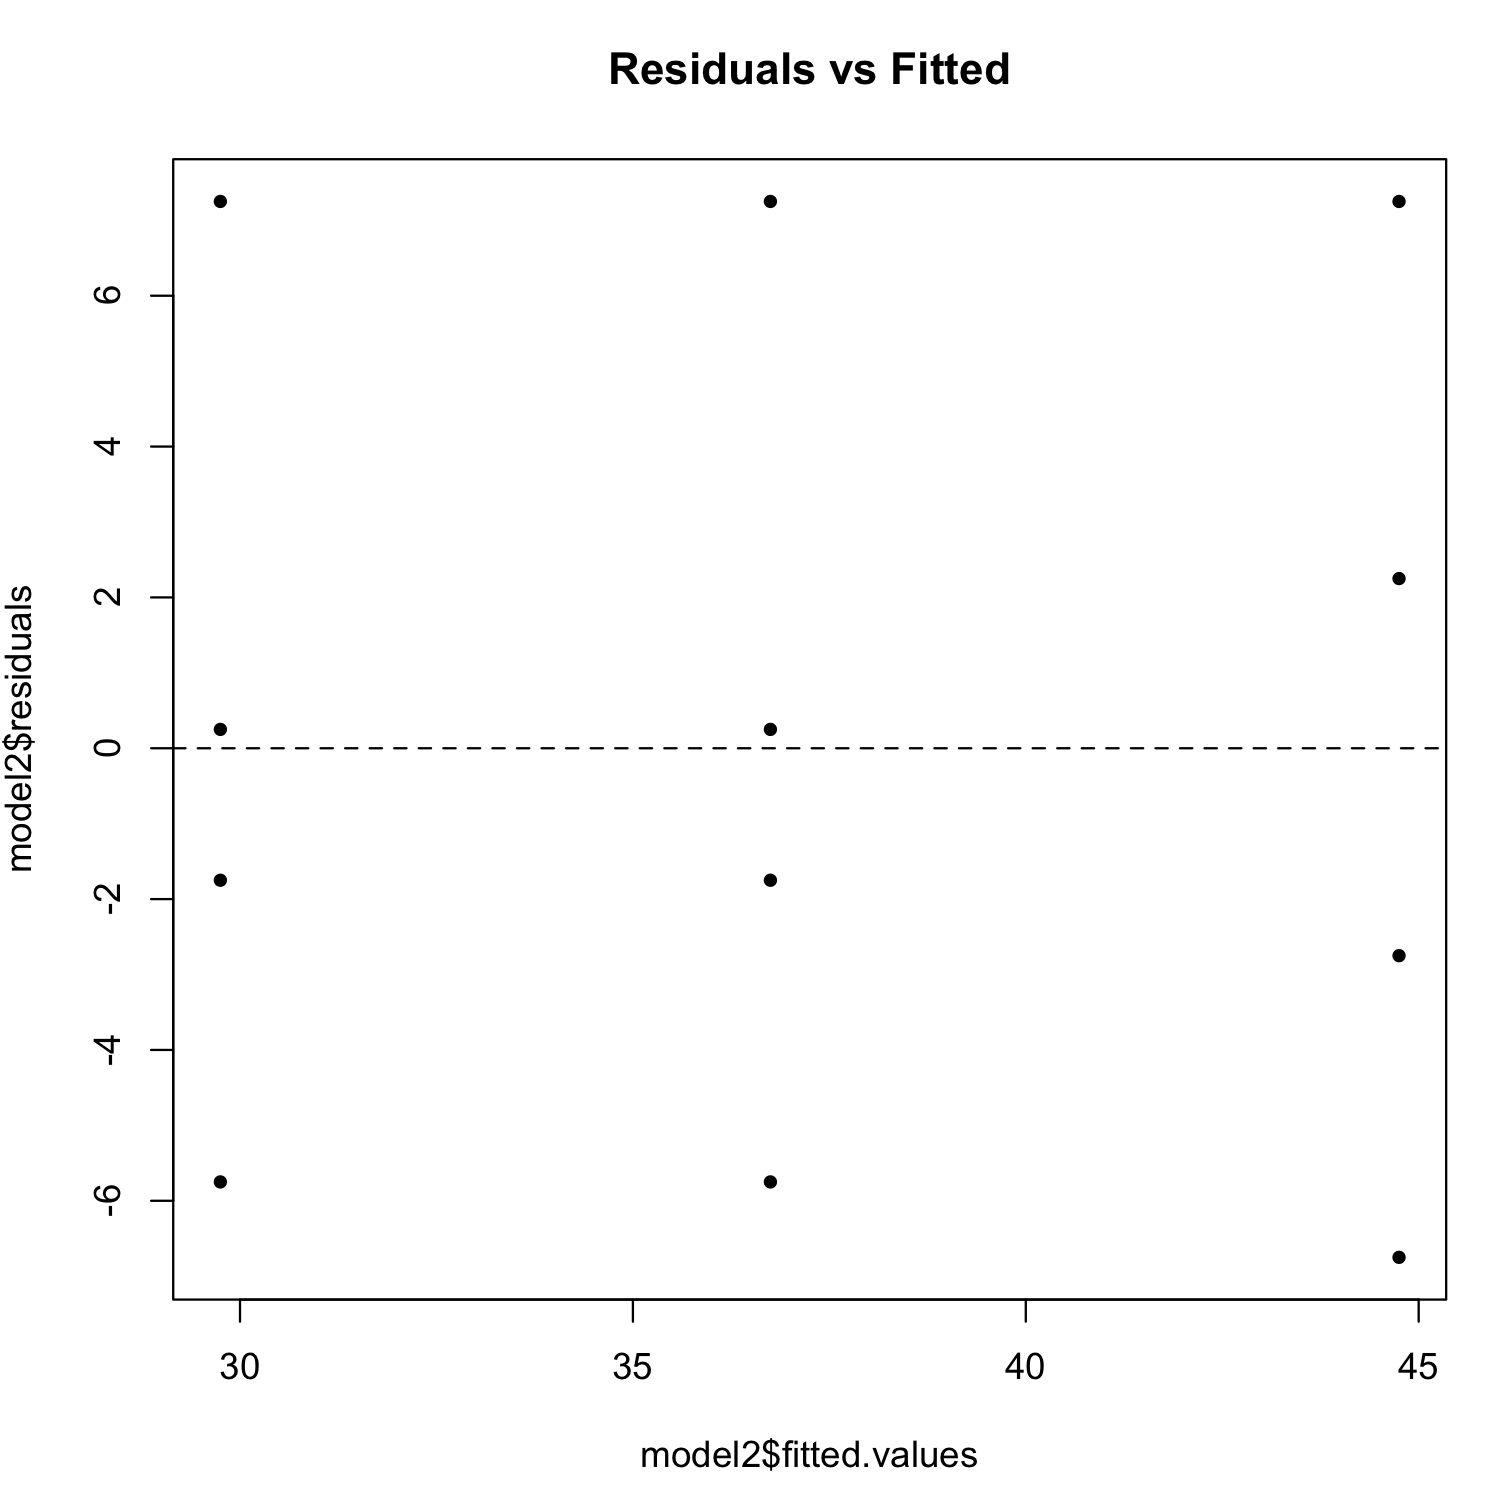
\includegraphics[width=\textwidth]{../pictures/hw2_q2_rf.png}
    \end{subfigure}
\end{figure}

There does not seem to be a problem with normality as the plots are generally in a straight line.
And the residuals are almost equally distributed around the 0 line without large outliers. Hence there is nothing too unusual about the residuals.

\end{document}

